\subsection{Mediciones}

Realizar una medición de performance \emph{rigurosa} es más difícil de lo 
que parece. 
En este experimento deberá realizar distintas mediciones de performance 
para verificar que sean buenas mediciones.

En un sistema ``ideal'' el proceso medido corre solo, sin ninguna 
interferencia de agentes externos. 
Sin embargo, una PC no es un sistema ideal. 
Nuestro proceso corre junto con decenas de otros, tanto de usuarios como 
del sistema operativo que compiten por el uso de la CPU. 
Esto implica que al realizar mediciones aparezcan ``ruidos'' o 
``interferencias'' que distorsionen los resultados.

El primer paso para tener una idea de si la medición es buena o no, 
es tomar varias muestras. 
Es decir, repetir la misma medición varias veces.
Luego de eso, es conveniente descartar los outliers
\footnote{en español, valor atípico: \url{http://es.wikipedia.org/wiki/Valor_atípico}}, 
que son los valores que más se alejan del promedio. 
Con los valores de las mediciones resultantes se puede calcular el promedio 
y también la varianza, que es algo similar el promedio de las distancias al 
promedio\footnote{en realidad, elevadas al cuadrado en vez de tomar el módulo}.

Las fórmulas para calcular el promedio $\mu$ y la varianza $\sigma^2$ son

$$
\mu = \frac{1}{n}\sum_{i=1}^{n} x_i \qquad \sigma^2 = \frac{\displaystyle\sum_{i=1}^{n}(x_i - \mu)^2} {n}
$$
%------------------------------------------

\subsection{Filtro \textit{cropflip}}

Programar el filtro \textit{cropflip} en lenguaje C y luego en ASM haciendo 
uso de las instrucciones vectoriales (\textbf{SSE}).

% ******************************************************************************
\vspace*{0.3cm} \noindent
\textbf{Experimento 1.1 - análisis el código generado}

En este experimento vamos a utilizar la herramienta \verb|objdump| para 
verificar como el compilador de C deja ensamblado el código C.

Ejecutar 
\begin{codesnippet}
\begin{verbatim}
objdump -Mintel -D cropflip_c.o
\end{verbatim}
\end{codesnippet}

¿Cómo es el código generado? 
Indicar
\begin{inparaenum}[\itshape a\upshape)]
    \item Por qué cree que hay otras funciones además de \verb|cropflip_c|
    \item Cómo se manipulan las variables locales
    \item Si le parece que ese código generado podría optimizarse
\end{inparaenum}

% ******************************************************************************
%\newpage
\vspace*{0.3cm} \noindent
\textbf{Experimento 1.2 - optimizaciones del compilador}

Compile el código de C con flags de optimización. Por ejemplo, pasando el flag 
\verb|-O1|\footnote{agregando este flag a \texttt{CCFLAGS64} en el makefile}. 
Indicar
\begin{inparaenum}
    \item Qué optimizaciones observa que realizó el compilador
    \item Qué otros flags de optimización brinda el compilador
    \item Los nombres de tres optimizaciones que realizan los compiladores.
\end{inparaenum}

%----------------------------------------------
\vspace*{0.3cm} \noindent
\textbf{Experimento 1.3 - calidad de las mediciones}

\begin{enumerate}
    \item Medir el tiempo de ejecución de cropflip 10 veces. Calcular el promedio y la varianza. Consideraremos outliers a los 2 mayores tiempos de ejecución de la medicion y también a los 2 menores, por lo que los descartaremos. Recalcular el promedio y la varianza después de hacer este descarte. Realizar un gráfico que presente estos dos últimos items.\\
\\
Luego de ejecutar 10 veces el filtro Cropflip obtuvimos los siguientes resultados: \\
\\
    	\begin{tabular}[c]{|c|c|c|}
	\hline
		\textbf{ASM} & \textbf{C}\\
		\hline
70.925 &	1.152.187\\
		\hline
70.521 &	1.151.544\\
		\hline
32.859 &	761.937\\
		\hline
43.720 &	649.248\\
		\hline
64.236 &	1.152.847\\
		\hline
70.793 &	1.153.061\\
		\hline
71.271 &	1.152.765\\
		\hline
44.616 &	1.152.798\\
		\hline
56.124 &	725.420\\
		\hline
71.775 &	1.155.718\\
		\hline
	\textbf{Esperanza}	\\
		\hline
59.684 & 1.020.752,5	\\
		\hline
		\textbf{Desvío standard}	\\
		\hline
13.720,5329 & 203.626,443	\\
		\hline
	\end{tabular}\\\\
	El cuadro denota la cantidad de ciclos de clock utilizada por cada ejecuci\'on del programa. \\
	\\
	Luego de eliminar los dos valores m\'as altos y los dos valores m\'as bajos, recalculamos obteniendo los siguientes datos: \\
	\textbf{Esperanza}: 62.869,166
 (ASM) y 1.087.346,333(C)\\
	\textbf{Desvío standard}:	9.719,205 (ASM) y 145.528,202(C)\\
	Se puede ver que al eliminar los outliers, la esperanza comienza a converger a su valor esperado y el desvío standard disminuye. \\
\\
\newpage
\begin{figure}
  \begin{center}
	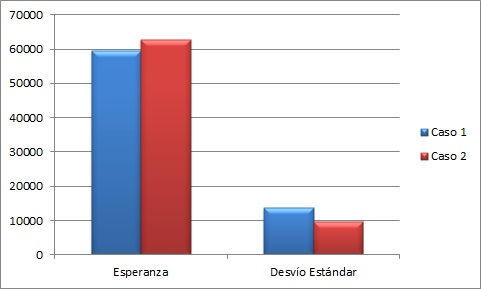
\includegraphics[width=0.7\textwidth]{imagenes/13/asm1.jpg}
	\caption{Assembler}
%	\label{nombreparareferenciar}
	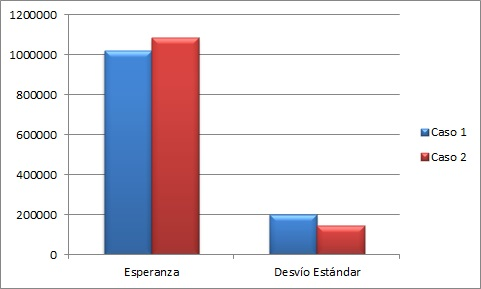
\includegraphics[width=0.7\textwidth]{imagenes/13/C1.jpg}
	\caption{C}
  \end{center}
\end{figure}
\newpage
\indent Siendo el Caso 1 las mediciones de esperanza y Desvío standard para todos los casos de test y el Caso 2 las mediciones sin tener en cuenta los cuatro outliers.\\
    \item Implementar un programa en C que no haga más que ciclar infinitamente sumando 1 a una variable. Lanzar este programa tantas veces como \emph{cores lógicos} tenga su procesador. Medir otras 10 veces mientras estos programas corren de fondo. Realizar los mismos casos de experimentaci\'on que en el ejercicio anterior.\\
\end{enumerate}
Los resultados obtenidos en esta experimentaci\'on fueron menores que los anteriores: \\
\\       
        \begin{tabular}[c]{|c|c|c|}
	\hline
		\textbf{ASM} & \textbf{C}\\
		\hline
33.585 &	542.928 \\
\hline
33.798 &	544.155 \\
\hline
33.402 &	544.857 \\
\hline
33.228 &	543.687 \\
\hline
33.159 &	543.252 \\
\hline
33.441 &	543.324 \\
\hline
34.089 &	544.224 \\ 
\hline
33.768 &	760.359 \\ 
\hline
34.563 &	542.448 \\
\hline
34.473 &	542.982 \\
\hline
		\textbf{Esperanza}	\\
		\hline
33.750,6 & 565.221,6	\\		
		\hline
		\textbf{Desvío standard}	\\
		\hline
465,49 & 65.049,34\\
		\hline
	\end{tabular}\\\\
	Luego de eliminar los dos valores m\'as altos y los dos valores m\'as bajos, recalculamos obteniendo los siguientes datos: \\
	\textbf{Esperanza}: 33.680,5 (ASM) y 543.604(C)\\
	\textbf{Desvío standard}:	235,364 (ASM) y 462,615(C)\\
	Ac\'a tambi\'en se puede apreciar que al eliminar los outliers, el Desvío standard disminuye su valor. \\
\newpage
\begin{figure}
  \begin{center}
	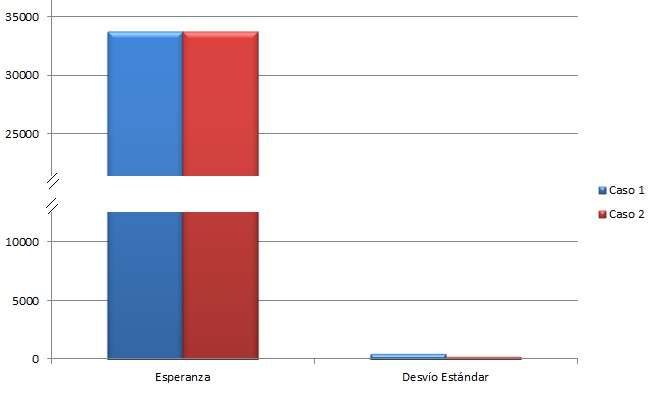
\includegraphics[width=0.7\textwidth]{imagenes/13/asm2.jpg}
	\caption{Assembler}
%	\label{nombreparareferenciar}
	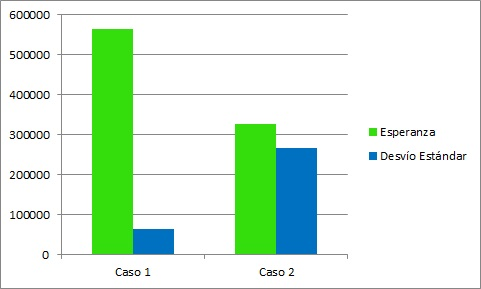
\includegraphics[width=0.7\textwidth]{imagenes/13/C2.jpg}
	\caption{C}
  \end{center}
\end{figure}
\newpage
\indent Siendo el Caso 1 las mediciones de esperanza y Desvío standard para todos los casos de test y el Caso 2 las mediciones sin tener en cuenta los cuatro outliers. Se puede observar que las mediciones mejoran con la ejecuci\'on del ciclo infinito de fondo, esto se debe a que fue ejecutado en una computadora con un procesador i5. \\
\\
\textit{A partir de aquí todos los experimentos de mediciones deberán hacerse igual 
que en el presente ejercicio: tomando 10 mediciones, luego descartando 
outliers y finalmente calculando promedio y Desvío standard.}\\
\\
Decidimos: \\
Realizar 12000 mediciones por experimento, eliminando los primeros mil casos que hayan llevado menos ciclos de clock y los mil casos que hayan llevado la mayor cantidad de ciclos de clock. \\
Lo determinamos de esta manera, ya que dejar dos mediciones afuera, como dice el enunciado, no tiene influencia en los c\'alculos de la esperanza y la varianza para muestras tan grandes. \\
Luego de experimentar distintas cantidades de casos de testeo, notamos que elegir 7000 valores pertenecientes a la franja del medio de los 12000 es una soluci\'on lo suficientemente establo, por lo cual es la que llevamos a cabo. \\
\\
% ******************************************************************************
%\newpage
\noindent\textbf{Experimento 1.4 - secuencial vs. vectorial}

En este experimento deberá realizar una medición de las diferencias de 
performance entre las versiones de C y ASM (el primero con -O0, -O1, -O2 y -O3) 
y graficar los resultados. \\
\\
El siguiente gr\'afico indica la esperanza de la cantidad de ciclos de clock que toma ejecutar el filtro Cropflip con los par\'ametros 404 404 4 4 en ASM y en C variando los flags de o0 a o3. \\
Reflejando las siguientes magnitudes: \\
\\
 \begin{tabular}[c]{|c|c|c|}
	\hline
		 & Esperanza & Desv\'io Standard\\
		\hline
C -o0 & 6.761.044,5 & 131,463 \\
\hline
C -o1 & 1.300.109 & 53,447 \\
\hline
C -o2 & 1.227.102,5 & 50,143\\
\hline
C -o3 & 266.688 & 0,287 \\
\hline
ASM & 362.232 & 2,079\\
\hline
	\end{tabular}\\\\
\\
Se puede observar que la varianza es casi despreciable considerando el valor de la esperanza. \\
\newpage
\begin{figure}
  \begin{center}
	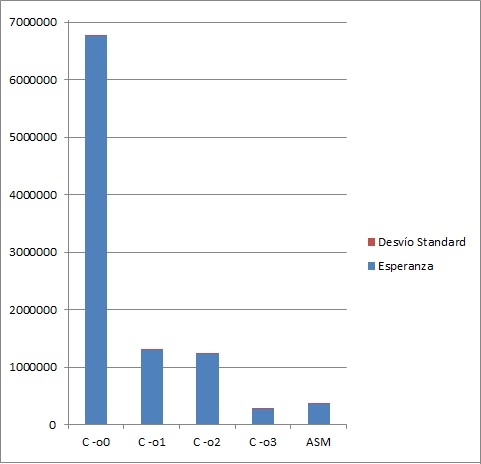
\includegraphics[width=0.7\textwidth]{imagenes/14.jpg}
  \end{center}
\end{figure}
\newpage

% ******************************************************************************
\vspace*{0.3cm} \noindent
\textbf{Experimento 1.5 - cpu vs. bus de memoria}

Se desea conocer cual es el mayor limitante a la
performance de este filtro en su versión ASM.

¿Cuál es el factor que limita la performance en este caso?
En caso de que el limitante fuera la intensidad de cómputo, entonces 
podrían agregarse instrucciones que realicen accesos a memoria extra y la
performance casi no debería sufrir. 
La inversa puede aplicarse, si el limitante es la cantidad de accesos a memoria.
\footnote{también podría pasar que estén más bien balanceados y que agregar
cualquier tipo de instrucción afecte sensiblemente la performance}
	
Realizar un experimento, agregando 4, 8 y 16 instrucciones aritméticas 
(por ej \verb|add rax, rbx|) analizando como varía el tiempo de ejecución.
Hacer lo mismo ahora con instrucciones de acceso a memoria, haciendo 
mitad lecturas y mitad escrituras (por ejemplo, agregando dos 
\verb|mov rax, [rsp]| y dos \verb|mov [rsp+8], rax|).\footnote{Notar que en el caso de acceder a \texttt{[rbp]} o \texttt{[rsp+8]} probablemente haya siempre hits en la cache, por lo que la medición no será de buena calidad. Si se le ocurre la manera, realizar accesos a otras direcciones alternativas.}
	
Realizar un único gráfico que compare:
\begin{inparaenum}
    \item La versión original
    \item Las versiones con más instrucciones aritméticas
    \item Las versiones com más accesos a memoria
\end{inparaenum}

Acompañar al gráfico con una tabla que indique los valores graficados.  
  
% ------------------------------------------------------------------------------

\subsection{Filtro \textit{Sierpinski}}

Programar el filtro \textit{Sierpinski} en lenguaje C y en en ASM haciendo 
uso de las instrucciones vectoriales (\textbf{SSE}).

% ******************************************************************************
\vspace*{0.3cm} \noindent
\textbf{Experimento 2.1 - secuencial vs. vectorial}

Analizar cuales son las diferencias de performace entre las versiones de C 
y ASM de este filtro, de igual modo que para el experimento 1.4. \\
\\
El siguiente gr\'afico indica la esperanza de la cantidad de ciclos de clock que toma ejecutar el filtro Sierpinski en ASM y en C variando los flags de o0 a o3. \\
Reflejando las siguientes magnitudes: \\
\\
 \begin{tabular}[c]{|c|c|c|}
	\hline
		 & Esperanza & Desv\'io Standard\\
		\hline
C -o0 & 28.801.586,5 & 78,016 \\
\hline
C -o1 & 21.395.732 & 78,447 \\
\hline
C -o2 & 14.231.758 & 116,445 \\
\hline
C -o3 & 14.229.650 & 116,022 \\
\hline
ASM & 3.661.626 & 115,583 \\
\hline
	\end{tabular}\\\\
\\
Aqu\'i tambi\'en el valor del desv\'io standard es despreciable. \\
\newpage
\begin{figure}
  \begin{center}
	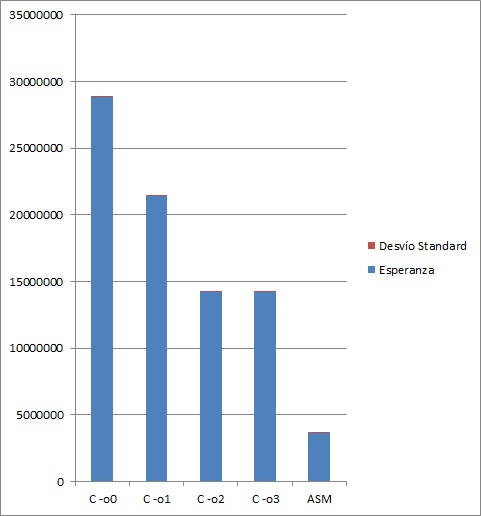
\includegraphics[width=0.7\textwidth]{imagenes/21.jpg}
  \end{center}
\end{figure}
\newpage

% ******************************************************************************
\vspace*{0.3cm} \noindent
\textbf{Experimento 2.1 - cpu vs. bus de memoria}

¿Cuál es el factor que limita la performance en este filtro?
Repetir el experimento 1.5 para este filtro.

\subsection{Filtro \textit{Bandas}}

Programar el filtro \textit{Bandas} en lenguaje C y en en ASM haciendo uso de 
las instrucciones vectoriales (\textbf{SSE}).

% ******************************************************************************
\vspace*{0.3cm} \noindent
\textbf{Experimento 3.1 - saltos condicionales}

Se desea conocer que tanto impactan los saltos condicionales en el código 
de filtro Bandas con \verb|-O1| (la versión en C).\\
Para poder medir esto de manera aproximada, remover el código
que detecta a que banda pertenece cada pixel, dejando
sólo una banda.
Por más que la imagen resultante no sea correcta, será posible tomar una
medida aproximada del impacto de los saltos condicionales.
Analizar como varía la performance. 

% ******************************************************************************
\vspace*{0.3cm} \noindent
\textbf{Experimento 3.2 - secuencial vs. vectorial}

Repetir el experimento 1.4 para este filtro. \\
\\
El siguiente gr\'afico indica la esperanza de la cantidad de ciclos de clock que toma ejecutar el filtro Bandas en ASM y en C variando los flags de o0 a o3. \\
Reflejando las siguientes magnitudes: \\
\\
 \begin{tabular}[c]{|c|c|c|}
	\hline
		 & Esperanza & Desv\'io Standard\\
		\hline
C -o0 & 17.472.791 & 120,620 \\
\hline
C -o1 & 4.583.340 & 128,514 \\
\hline
C -o2 & 3.259.839 & 117,746 \\
\hline
C -o3 & 3.259.767 & 117,391  \\
\hline
ASM & 3.703.203,5 & 115,659 \\
\hline
	\end{tabular}\\\\
\\
Aqu\'i tambi\'en el valor del desv\'io standard es despreciable. \\
\newpage
\begin{figure}
  \begin{center}
	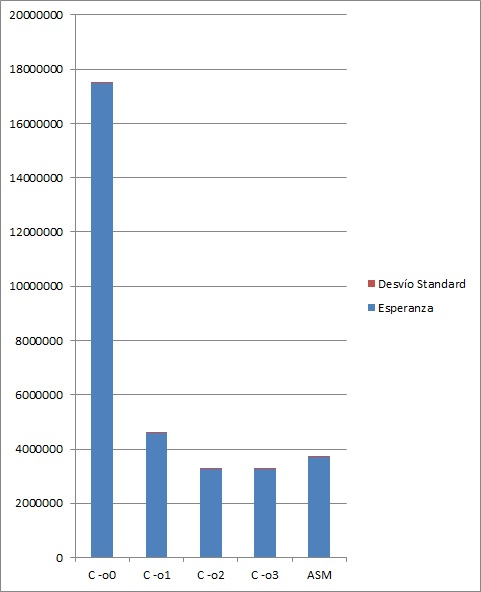
\includegraphics[width=0.7\textwidth]{imagenes/32.jpg}
  \end{center}
\end{figure}
\newpage

% ------------------------------------------------------------------------------

\subsection{Filtro \textit{Motion Blur}}
Programar el filtro \textit{mblur} en lenguaje C y en ASM haciendo uso de 
las instrucciones \textbf{SSE}.

% ******************************************************************************
\vspace*{0.3cm} \noindent
\textbf{Experimento 4.1}

Repetir el experimento 1.4 para este filtro \\
\\
El siguiente gr\'afico indica la esperanza de la cantidad de ciclos de clock que toma ejecutar el filtro Bandas en ASM y en C variando los flags de o0 a o3. \\
Reflejando las siguientes magnitudes: \\
\\
 \begin{tabular}[c]{|c|c|c|}
	\hline
		 & Esperanza & Desv\'io Standard\\
		\hline
C -o0 & 24.652.732,5 & 117,738 \\
\hline
C -o1 & 11.562.261 & 103,024  \\
\hline
C -o2 & 9.641.346 & 78,159  \\
\hline
C -o3 & 9.639.625 & 78,227 \\
\hline
ASM & 2.993.980,5 & 118,245 \\
\hline
	\end{tabular}\\\\
\\
Aqu\'i tambi\'en el valor del desv\'io standard es despreciable. \\
\newpage
\begin{figure}
  \begin{center}
	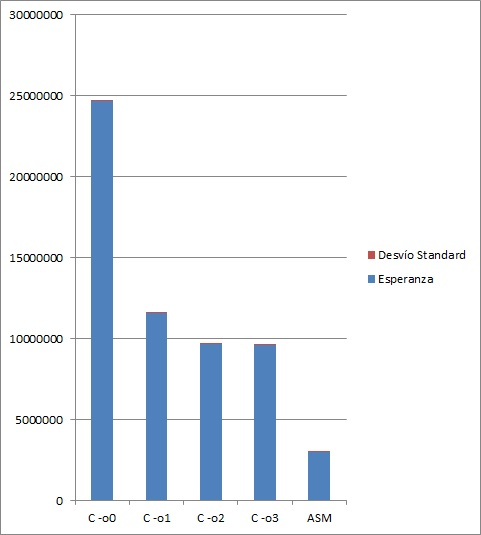
\includegraphics[width=0.7\textwidth]{imagenes/41.jpg}
  \end{center}
\end{figure}
\newpage